
\section{Additional Ablation Studies}
\begin{figure}[!]
    \centering
    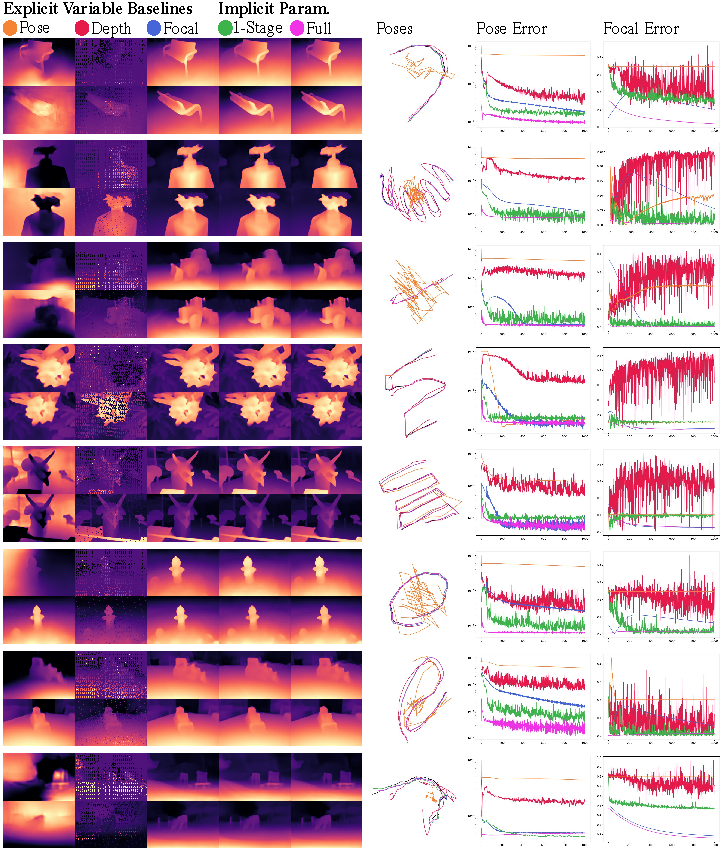
\includegraphics[width=\linewidth,]{figures/pdfs/source_matrix_large_compressed.pdf}
    \caption{\textbf{Pose and Geometry Convergence for Free-Variable vs. Proposed Parameterizations.}
    We plot poses, depths, focal lengths, and pose error (ATE) obtained with our proposed parameterizations (``Full'') vs. those obtained with free-variable parameterizations at various optimization steps. With our proposed reparameterizations (``Full'') as a baseline, we ablate either depth, focal length, or poses as free-variable optimizations and plot the resulting optimizations' pose and depth estimates. For instance, ``Depth'' corresponds to making the depth an explicit free-variable in the optimization. Using pose-as-variable and depth-as-variable often lead to ``hollow-face'' geometry, where the geometry is effectively inverted but still mostly satisfies the optical flow constraints. We also show results from a single-stage FlowMap pipeline, which only uses the implicit parameterization of intrinsics rather than switching to regressed intrinsics halfway through optimization. Note that the plotted lines for ``Full'' are initialized with the results of ``1-Stage'' and represent the second stage (explicit focal length) of FlowMap optimization.}
    \label{fig:convergence}
\end{figure}

\setlength{\tabcolsep}{8pt}
\begin{table*}[t]

\centering

\newcommand{\first}{\cellcolor{red!40}}
\newcommand{\second}{\cellcolor{orange!40}}
\newcommand{\third}{\cellcolor{yellow!40}}
\setlength{\tabcolsep}{4pt}

\begin{tabular}{lrrr}
\toprule
Method              & PSNR $\uparrow$ & SSIM $\uparrow$ & LPIPS $\downarrow$ \\
\midrule
FlowMap             &   \first{27.70} &   \first{0.863} &      \first{0.089} \\
Single Stage        &   \third{26.66} &   \third{0.842} &      \third{0.112} \\
Expl. Focal Length  &           25.15 &           0.788 &              0.141 \\
Expl. Depth         &            8.84 &           0.168 &              0.684 \\
Expl. Pose          &           16.00 &           0.533 &              0.495 \\
No Tracks           &           25.83 &           0.822 &              0.122 \\
Random Init.        &           25.54 &           0.808 &              0.129 \\
Random Init. (20k)  &  \second{27.25} &  \second{0.850} &     \second{0.101} \\
No Corresp. Weights &           24.18 &           0.765 &              0.168 \\
\bottomrule
\end{tabular}

\vspace{10pt}

\caption{\textbf{Additional Ablations.} We report additional ablation results averaged across all scenes alongside the ablations found in the main paper.}

\label{tab:ablations_supplemental}
\end{table*}

\setlength{\tabcolsep}{8pt}
\begin{table*}[t]

\newcommand{\first}{\cellcolor{red!40}}
\newcommand{\second}{\cellcolor{orange!40}}
\newcommand{\third}{\cellcolor{yellow!40}}
\setlength{\tabcolsep}{4pt}

\centering
\resizebox{\textwidth}{!}{

\begin{tabular}{l|rrrrr|rrrrr|rrrrr}
\toprule
\multicolumn{1}{c|}{} & \multicolumn{5}{|c|}{Fern (LLFF)} & \multicolumn{5}{|c|}{Flower (LLFF)} & \multicolumn{5}{|c}{Fortress (LLFF)} \\
\midrule
Method              & PSNR $\uparrow$ & SSIM $\uparrow$ & LPIPS $\downarrow$ & Time (min.) $\downarrow$ & ATE     & PSNR $\uparrow$ & SSIM $\uparrow$ & LPIPS $\downarrow$ & Time (min.) $\downarrow$ & ATE     & PSNR $\uparrow$ & SSIM $\uparrow$ & LPIPS $\downarrow$ & Time (min.) $\downarrow$ & ATE     \\
\midrule
FlowMap             &   \first{23.70} &   \first{0.801} &      \first{0.096} &                      4.8 & 0.00233 &           29.07 &   \third{0.877} &      \third{0.084} &                      6.6 & 0.00079 &   \first{31.13} &   \third{0.906} &              0.060 &                      7.8 & 0.00049 \\
Single Stage        &  \second{23.64} &  \second{0.797} &     \second{0.098} &                      4.9 & 0.00294 &           29.06 &   \third{0.877} &              0.086 &                      6.7 & 0.00065 &  \second{31.05} &  \second{0.908} &     \second{0.058} &                      7.9 & 0.00054 \\
Expl. Focal Length  &           23.07 &           0.787 &              0.119 &                      4.6 & 0.00296 &   \third{29.13} &           0.874 &      \first{0.079} &                      6.4 & 0.00293 &           29.82 &           0.891 &              0.062 &                      7.6 & 0.00223 \\
Expl. Depth         &            4.71 &           0.001 &              0.785 &              \first{2.9} & 0.00785 &            8.04 &           0.007 &              0.839 &              \first{3.6} & 0.00666 &            2.60 &           0.001 &              0.774 &              \first{4.1} & 0.00664 \\
Expl. Pose          &            4.71 &           0.001 &              0.785 &                      4.5 & 0.01118 &           15.51 &           0.569 &              0.428 &                      6.3 & 0.00192 &           16.49 &           0.577 &              0.594 &                      7.4 & 0.01302 \\
No Tracks           &   \third{23.58} &   \third{0.796} &      \third{0.099} &             \second{4.3} & 0.00316 &  \second{29.29} &  \second{0.879} &      \third{0.084} &             \second{5.5} & 0.00337 &           30.92 &   \third{0.906} &      \third{0.059} &             \second{6.3} & 0.00143 \\
Random Init.        &           22.68 &           0.756 &              0.113 &                      4.8 & 0.00371 &           28.47 &           0.864 &      \third{0.084} &                      6.6 & 0.00303 &           30.96 &           0.904 &      \third{0.059} &                      7.8 & 0.00068 \\
Random Init. (20k)  &           23.50 &           0.791 &     \second{0.098} &                     44.2 & 0.00312 &   \first{29.33} &   \first{0.880} &     \second{0.083} &                     59.4 & 0.00054 &   \third{31.04} &   \first{0.911} &      \first{0.057} &                     69.7 & 0.00047 \\
No Corresp. Weights &           23.27 &           0.784 &              0.104 &              \third{4.4} & 0.00311 &           27.61 &           0.844 &              0.090 &              \third{6.0} & 0.00554 &           24.05 &           0.709 &              0.138 &              \third{7.1} & 0.01363 \\
\midrule
\multicolumn{1}{c|}{} & \multicolumn{5}{|c|}{Horns (LLFF)} & \multicolumn{5}{|c|}{Orchids (LLFF)} & \multicolumn{5}{|c}{Room (LLFF)} \\
\midrule
Method              & PSNR $\uparrow$ & SSIM $\uparrow$ & LPIPS $\downarrow$ & Time (min.) $\downarrow$ & ATE     & PSNR $\uparrow$ & SSIM $\uparrow$ & LPIPS $\downarrow$ & Time (min.) $\downarrow$ & ATE     & PSNR $\uparrow$ & SSIM $\uparrow$ & LPIPS $\downarrow$ & Time (min.) $\downarrow$ & ATE     \\
\midrule
FlowMap             &   \first{28.35} &   \first{0.903} &     \second{0.071} &                     10.6 & 0.00049 &           19.16 &           0.615 &      \third{0.132} &                      5.5 & 0.00127 &   \first{32.93} &  \second{0.958} &      \first{0.037} &                      7.8 & 0.00274 \\
Single Stage        &           28.19 &   \third{0.899} &     \second{0.071} &                     10.7 & 0.00051 &  \second{19.33} &  \second{0.623} &     \second{0.129} &                      5.6 & 0.00120 &  \second{32.75} &   \first{0.959} &      \first{0.037} &                      7.9 & 0.00265 \\
Expl. Focal Length  &           24.57 &           0.823 &              0.153 &                     10.5 & 0.00100 &           18.96 &           0.606 &              0.151 &                      5.3 & 0.00184 &   \third{32.13} &   \third{0.953} &     \second{0.040} &                      7.6 & 0.00274 \\
Expl. Depth         &            5.94 &           0.002 &              0.788 &              \first{5.3} & 0.00603 &            6.25 &           0.003 &              0.886 &              \first{3.2} & 0.00647 &            5.78 &           0.004 &              0.616 &              \first{4.1} & 0.00710 \\
Expl. Pose          &           14.66 &           0.506 &              0.685 &                     10.0 & 0.01230 &           12.80 &           0.279 &              0.429 &                      5.2 & 0.01496 &           16.92 &           0.767 &              0.466 &                      7.3 & 0.00596 \\
No Tracks           &   \third{28.32} &  \second{0.900} &     \second{0.071} &             \second{8.2} & 0.00173 &   \third{19.21} &   \third{0.616} &              0.133 &             \second{4.8} & 0.00195 &           28.98 &           0.922 &              0.068 &             \second{6.3} & 0.00938 \\
Random Init.        &           23.93 &           0.729 &              0.172 &                     10.6 & 0.00486 &           18.85 &           0.594 &              0.146 &                      5.4 & 0.00188 &           29.19 &           0.920 &              0.067 &                      7.8 & 0.00422 \\
Random Init. (20k)  &  \second{28.33} &  \second{0.900} &      \first{0.068} &                     94.2 & 0.00054 &   \first{19.40} &   \first{0.629} &      \first{0.126} &                     49.5 & 0.00112 &           31.92 &           0.949 &              0.043 &                     69.4 & 0.00288 \\
No Corresp. Weights &           28.17 &           0.893 &      \third{0.072} &              \third{9.6} & 0.00169 &           18.76 &           0.597 &              0.148 &              \third{5.1} & 0.00307 &           31.81 &           0.952 &      \third{0.041} &              \third{7.1} & 0.00331 \\
\midrule
\multicolumn{1}{c|}{} & \multicolumn{5}{|c|}{Trex (LLFF)} & \multicolumn{5}{|c|}{Bonsai (MipNeRF 360)} & \multicolumn{5}{|c}{Kitchen (MipNeRF 360)} \\
\midrule
Method              & PSNR $\uparrow$ & SSIM $\uparrow$ & LPIPS $\downarrow$ & Time (min.) $\downarrow$ & ATE     & PSNR $\uparrow$ & SSIM $\uparrow$ & LPIPS $\downarrow$ & Time (min.) $\downarrow$ & ATE     & PSNR $\uparrow$ & SSIM $\uparrow$ & LPIPS $\downarrow$ & Time (min.) $\downarrow$ & ATE     \\
\midrule
FlowMap             &   \third{26.27} &   \third{0.880} &     \second{0.075} &                      9.7 & 0.00655 &   \first{32.24} &  \second{0.950} &      \first{0.047} &                     24.2 & 0.00048 &  \second{30.47} &  \second{0.936} &     \second{0.049} &                     10.9 & 0.00041 \\
Single Stage        &   \first{26.65} &   \first{0.886} &      \first{0.073} &                      9.8 & 0.00655 &  \second{32.21} &   \first{0.951} &     \second{0.048} &                     24.3 & 0.00046 &   \third{30.26} &   \third{0.925} &      \third{0.051} &                     11.1 & 0.00072 \\
Expl. Focal Length  &           24.57 &           0.852 &              0.107 &                      9.5 & 0.00766 &           21.36 &           0.689 &              0.231 &                     24.1 & 0.00184 &           21.29 &           0.645 &              0.174 &                     10.7 & 0.00449 \\
Expl. Depth         &            5.56 &           0.002 &              0.759 &              \first{4.8} & 0.04406 &           10.46 &           0.045 &              0.633 &             \first{11.3} & 0.02830 &            5.08 &           0.016 &              0.753 &              \first{5.3} & 0.00827 \\
Expl. Pose          &           15.09 &           0.540 &              0.544 &                      9.2 & 0.02277 &           13.12 &           0.425 &              0.577 &                     22.8 & 0.01407 &           14.18 &           0.387 &              0.587 &                     10.3 & 0.01669 \\
No Tracks           &           24.36 &           0.831 &              0.110 &             \second{7.8} & 0.02011 &           25.53 &   \third{0.863} &      \third{0.115} &            \second{18.0} & 0.00291 &           25.48 &           0.794 &              0.112 &             \second{8.5} & 0.00302 \\
Random Init.        &           24.84 &           0.835 &              0.099 &                      9.7 & 0.00598 &           18.38 &           0.585 &              0.342 &                     24.2 & 0.01380 &           24.94 &           0.764 &              0.113 &                     10.9 & 0.00345 \\
Random Init. (20k)  &  \second{26.45} &  \second{0.882} &      \third{0.076} &                     86.5 & 0.00991 &           18.75 &           0.600 &              0.342 &                    214.8 & 0.01433 &   \first{31.69} &   \first{0.945} &      \first{0.044} &                     96.8 & 0.00023 \\
No Corresp. Weights &           25.33 &           0.859 &              0.094 &              \third{8.8} & 0.01083 &   \third{25.59} &           0.841 &              0.118 &             \third{21.8} & 0.00141 &           24.62 &           0.742 &              0.118 &              \third{9.9} & 0.00422 \\
\midrule
\multicolumn{1}{c|}{} & \multicolumn{5}{|c|}{Counter (MipNeRF 360)} & \multicolumn{5}{|c|}{Barn (Tanks \& Temples)} & \multicolumn{5}{|c}{Caterpillar (Tanks \& Temples)} \\
\midrule
Method              & PSNR $\uparrow$ & SSIM $\uparrow$ & LPIPS $\downarrow$ & Time (min.) $\downarrow$ & ATE     & PSNR $\uparrow$ & SSIM $\uparrow$ & LPIPS $\downarrow$ & Time (min.) $\downarrow$ & ATE     & PSNR $\uparrow$ & SSIM $\uparrow$ & LPIPS $\downarrow$ & Time (min.) $\downarrow$ & ATE     \\
\midrule
FlowMap             &  \second{26.80} &  \second{0.862} &     \second{0.121} &                     24.2 & 0.00076 &   \first{27.10} &  \second{0.872} &     \second{0.090} &                     22.3 & 0.00048 &  \second{28.25} &  \second{0.830} &     \second{0.113} &                     22.3 & 0.00030 \\
Single Stage        &   \third{26.65} &   \third{0.857} &      \third{0.124} &                     24.3 & 0.00083 &           26.28 &           0.857 &              0.104 &                     22.4 & 0.00102 &   \first{28.32} &   \first{0.834} &      \first{0.110} &                     22.4 & 0.00026 \\
Expl. Focal Length  &           21.82 &           0.697 &              0.237 &                     24.1 & 0.00355 &  \second{27.04} &   \first{0.873} &      \first{0.086} &                     21.9 & 0.00085 &           27.12 &           0.789 &              0.133 &                     22.1 & 0.00046 \\
Expl. Depth         &            8.80 &           0.029 &              0.719 &             \first{11.4} & 0.01003 &           17.01 &           0.591 &              0.489 &             \first{10.7} & 0.00923 &            9.15 &           0.016 &              0.732 &             \first{10.7} & 0.00841 \\
Expl. Pose          &           14.40 &           0.506 &              0.554 &                     22.9 & 0.00611 &           18.09 &           0.625 &              0.455 &                     20.9 & 0.02160 &           17.57 &           0.491 &              0.554 &                     21.1 & 0.00817 \\
No Tracks           &           23.91 &           0.788 &              0.183 &            \second{18.1} & 0.00240 &           25.41 &           0.837 &              0.122 &            \second{16.1} & 0.00363 &           27.33 &           0.807 &              0.133 &            \second{16.1} & 0.00095 \\
Random Init.        &           26.05 &           0.847 &              0.131 &                     24.2 & 0.00088 &           26.24 &           0.864 &              0.100 &                     22.2 & 0.00079 &           26.27 &           0.750 &              0.169 &                     22.2 & 0.00147 \\
Random Init. (20k)  &   \first{26.88} &   \first{0.867} &      \first{0.115} &                    214.3 & 0.00064 &   \third{26.80} &   \third{0.871} &      \third{0.091} &                    197.3 & 0.00049 &   \third{28.01} &   \third{0.823} &      \third{0.122} &                    197.3 & 0.00031 \\
No Corresp. Weights &           17.93 &           0.575 &              0.391 &             \third{21.8} & 0.01099 &           24.53 &           0.820 &              0.133 &             \third{20.3} & 0.00244 &           25.93 &           0.734 &              0.174 &             \third{20.1} & 0.00106 \\
\midrule
\multicolumn{1}{c|}{} & \multicolumn{5}{|c|}{Church (Tanks \& Temples)} & \multicolumn{5}{|c|}{Courthouse (Tanks \& Temples)} & \multicolumn{5}{|c}{Family (Tanks \& Temples)} \\
\midrule
Method              & PSNR $\uparrow$ & SSIM $\uparrow$ & LPIPS $\downarrow$ & Time (min.) $\downarrow$ & ATE     & PSNR $\uparrow$ & SSIM $\uparrow$ & LPIPS $\downarrow$ & Time (min.) $\downarrow$ & ATE     & PSNR $\uparrow$ & SSIM $\uparrow$ & LPIPS $\downarrow$ & Time (min.) $\downarrow$ & ATE     \\
\midrule
FlowMap             &  \second{28.29} &  \second{0.883} &      \first{0.074} &                     22.4 & 0.00061 &   \third{27.51} &  \second{0.911} &     \second{0.055} &                     22.2 & 0.00129 &  \second{27.96} &  \second{0.889} &     \second{0.067} &                     22.1 & 0.00039 \\
Single Stage        &           27.60 &   \third{0.875} &     \second{0.079} &                     22.3 & 0.00061 &   \first{27.67} &   \first{0.914} &      \first{0.054} &                     22.3 & 0.00150 &   \third{27.65} &   \third{0.880} &      \third{0.075} &                     22.4 & 0.00033 \\
Expl. Focal Length  &           27.29 &           0.856 &              0.088 &                     22.0 & 0.00093 &           26.86 &   \third{0.897} &      \third{0.069} &                     22.1 & 0.00234 &           27.10 &           0.873 &              0.082 &                     22.0 & 0.00082 \\
Expl. Depth         &           16.21 &           0.518 &              0.474 &             \first{10.7} & 0.02314 &            3.52 &           0.001 &              0.745 &             \first{10.7} & 0.00718 &            4.09 &           0.001 &              0.773 &             \first{10.8} & 0.01403 \\
Expl. Pose          &           17.66 &           0.582 &              0.457 &                     21.0 & 0.00807 &           19.68 &           0.726 &              0.251 &                     21.0 & 0.00511 &           15.79 &           0.562 &              0.507 &                     21.1 & 0.03074 \\
No Tracks           &           26.93 &           0.851 &              0.100 &            \second{16.1} & 0.00259 &           25.27 &           0.858 &              0.108 &            \second{16.1} & 0.00442 &           27.00 &           0.869 &              0.088 &            \second{16.1} & 0.00172 \\
Random Init.        &           27.45 &           0.858 &              0.089 &                     22.2 & 0.00112 &           26.55 &           0.894 &              0.071 &                     22.2 & 0.00314 &           26.36 &           0.858 &              0.093 &                     22.2 & 0.00148 \\
Random Init. (20k)  &   \first{28.67} &   \first{0.886} &      \first{0.074} &                    197.4 & 0.00030 &  \second{27.62} &  \second{0.911} &      \first{0.054} &                    197.8 & 0.00101 &   \first{28.07} &   \first{0.892} &      \first{0.066} &                    196.9 & 0.00019 \\
No Corresp. Weights &   \third{27.86} &   \third{0.875} &      \third{0.081} &             \third{20.3} & 0.00086 &           25.62 &           0.868 &              0.086 &             \third{20.1} & 0.00264 &           19.01 &           0.629 &              0.313 &             \third{20.2} & 0.00672 \\
\midrule
\multicolumn{1}{c|}{} & \multicolumn{5}{|c|}{Francis (Tanks \& Temples)} & \multicolumn{5}{|c|}{Horse (Tanks \& Temples)} & \multicolumn{5}{|c}{Ignatius (Tanks \& Temples)} \\
\midrule
Method              & PSNR $\uparrow$ & SSIM $\uparrow$ & LPIPS $\downarrow$ & Time (min.) $\downarrow$ & ATE     & PSNR $\uparrow$ & SSIM $\uparrow$ & LPIPS $\downarrow$ & Time (min.) $\downarrow$ & ATE     & PSNR $\uparrow$ & SSIM $\uparrow$ & LPIPS $\downarrow$ & Time (min.) $\downarrow$ & ATE     \\
\midrule
FlowMap             &  \second{31.90} &  \second{0.903} &     \second{0.080} &                     22.4 & 0.00058 &   \first{28.35} &   \first{0.917} &      \first{0.064} &                     22.4 & 0.00054 &   \first{24.54} &   \first{0.773} &      \first{0.131} &                     22.4 & 0.00037 \\
Single Stage        &   \first{32.20} &   \first{0.905} &      \first{0.078} &                     22.4 & 0.00054 &           11.42 &           0.635 &              0.496 &                     22.3 & 0.03959 &  \second{24.48} &   \third{0.764} &      \first{0.131} &                     22.4 & 0.00024 \\
Expl. Focal Length  &           30.89 &           0.884 &              0.108 &                     22.0 & 0.00040 &   \third{27.82} &   \third{0.905} &      \third{0.074} &                     22.0 & 0.00102 &           23.12 &           0.723 &      \third{0.157} &                     22.0 & 0.00071 \\
Expl. Depth         &            7.42 &           0.006 &              0.631 &             \first{10.8} & 0.01956 &            2.67 &           0.000 &              0.691 &             \first{10.7} & 0.02555 &            5.68 &           0.006 &              0.867 &             \first{10.7} & 0.02181 \\
Expl. Pose          &           18.19 &           0.639 &              0.464 &                     20.9 & 0.03102 &           14.60 &           0.661 &              0.468 &                     21.0 & 0.03918 &           12.48 &           0.314 &              0.640 &                     20.9 & 0.02886 \\
No Tracks           &           30.72 &           0.887 &              0.100 &            \second{16.1} & 0.00113 &           25.50 &           0.882 &              0.101 &            \second{16.1} & 0.00241 &           23.54 &           0.727 &              0.163 &            \second{16.1} & 0.00144 \\
Random Init.        &           29.44 &           0.862 &              0.122 &                     22.3 & 0.00289 &           25.07 &           0.871 &              0.119 &                     22.2 & 0.00380 &           23.50 &           0.737 &              0.159 &                     22.1 & 0.00084 \\
Random Init. (20k)  &   \third{31.56} &   \third{0.899} &      \third{0.085} &                    197.7 & 0.00138 &  \second{28.16} &  \second{0.915} &     \second{0.067} &                    197.0 & 0.00066 &   \third{24.47} &  \second{0.771} &     \second{0.133} &                    197.5 & 0.00034 \\
No Corresp. Weights &           28.92 &           0.850 &              0.130 &             \third{20.1} & 0.00397 &           25.82 &           0.871 &              0.100 &             \third{20.2} & 0.00275 &           21.89 &           0.655 &              0.197 &             \third{20.2} & 0.00108 \\
\midrule
\multicolumn{1}{c|}{} & \multicolumn{5}{|c|}{M60 (Tanks \& Temples)} & \multicolumn{5}{|c|}{Museum (Tanks \& Temples)} & \multicolumn{5}{|c}{Panther (Tanks \& Temples)} \\
\midrule
Method              & PSNR $\uparrow$ & SSIM $\uparrow$ & LPIPS $\downarrow$ & Time (min.) $\downarrow$ & ATE     & PSNR $\uparrow$ & SSIM $\uparrow$ & LPIPS $\downarrow$ & Time (min.) $\downarrow$ & ATE     & PSNR $\uparrow$ & SSIM $\uparrow$ & LPIPS $\downarrow$ & Time (min.) $\downarrow$ & ATE     \\
\midrule
FlowMap             &   \third{23.23} &  \second{0.805} &      \third{0.190} &                     22.4 & 0.00838 &   \third{28.48} &   \third{0.862} &      \third{0.078} &                     22.2 & 0.00070 &  \second{27.50} &  \second{0.882} &     \second{0.105} &                     22.3 & 0.00112 \\
Single Stage        &  \second{23.30} &   \third{0.803} &     \second{0.187} &                     22.3 & 0.00832 &  \second{28.62} &  \second{0.866} &     \second{0.076} &                     22.4 & 0.00058 &   \third{27.31} &   \third{0.881} &      \first{0.104} &                     22.4 & 0.00118 \\
Expl. Focal Length  &           19.65 &           0.696 &              0.278 &                     22.1 & 0.01400 &           28.15 &           0.850 &              0.092 &                     22.0 & 0.00124 &           21.86 &           0.737 &              0.239 &                     22.1 & 0.00893 \\
Expl. Depth         &           13.65 &           0.529 &              0.547 &             \first{10.7} & 0.01945 &           16.55 &           0.507 &              0.489 &             \first{10.7} & 0.03144 &           16.17 &           0.619 &              0.456 &             \first{10.5} & 0.01527 \\
Expl. Pose          &           14.37 &           0.566 &              0.546 &                     21.1 & 0.01454 &           16.12 &           0.489 &              0.524 &                     21.1 & 0.03128 &           16.41 &           0.613 &              0.460 &                     20.9 & 0.00523 \\
No Tracks           &           23.17 &  \second{0.805} &              0.195 &            \second{16.1} & 0.00674 &           27.63 &           0.844 &              0.096 &            \second{16.1} & 0.00150 &           24.69 &           0.833 &              0.161 &            \second{16.1} & 0.00605 \\
Random Init.        &           21.81 &           0.781 &              0.206 &                     22.3 & 0.01008 &           27.57 &           0.849 &              0.094 &                     22.3 & 0.00108 &           25.25 &           0.845 &              0.141 &                     22.2 & 0.00352 \\
Random Init. (20k)  &   \first{23.61} &   \first{0.817} &      \first{0.171} &                    197.7 & 0.00869 &   \first{28.74} &   \first{0.868} &      \first{0.075} &                    196.9 & 0.00067 &   \first{27.61} &   \first{0.884} &     \second{0.105} &                    198.1 & 0.00131 \\
No Corresp. Weights &            9.44 &           0.545 &              0.651 &             \third{20.2} & 0.02315 &           27.94 &           0.849 &              0.086 &             \third{20.1} & 0.00122 &           26.00 &           0.850 &      \third{0.138} &             \third{20.0} & 0.00182 \\
\midrule
\multicolumn{1}{c|}{} & \multicolumn{5}{|c|}{Playground (Tanks \& Temples)} & \multicolumn{5}{|c|}{Train (Tanks \& Temples)} & \multicolumn{5}{|c}{Truck (Tanks \& Temples)} \\
\midrule
Method              & PSNR $\uparrow$ & SSIM $\uparrow$ & LPIPS $\downarrow$ & Time (min.) $\downarrow$ & ATE     & PSNR $\uparrow$ & SSIM $\uparrow$ & LPIPS $\downarrow$ & Time (min.) $\downarrow$ & ATE     & PSNR $\uparrow$ & SSIM $\uparrow$ & LPIPS $\downarrow$ & Time (min.) $\downarrow$ & ATE     \\
\midrule
FlowMap             &   \first{24.29} &   \first{0.727} &      \first{0.192} &                     22.2 & 0.00096 &  \second{26.22} &  \second{0.870} &     \second{0.077} &                     22.2 & 0.00082 &   \first{24.34} &   \first{0.828} &      \first{0.098} &                     22.3 & 0.00078 \\
Single Stage        &  \second{23.39} &  \second{0.710} &     \second{0.209} &                     22.4 & 0.00102 &   \third{26.11} &   \third{0.863} &      \third{0.082} &                     22.3 & 0.00100 &           24.21 &  \second{0.826} &     \second{0.102} &                     22.3 & 0.00074 \\
Expl. Focal Length  &           18.55 &           0.525 &              0.380 &                     21.9 & 0.00621 &           25.82 &           0.847 &              0.092 &                     22.1 & 0.00199 &           24.03 &           0.816 &              0.110 &                     22.0 & 0.00070 \\
Expl. Depth         &           14.29 &           0.427 &              0.637 &             \first{10.6} & 0.01642 &           15.89 &           0.553 &              0.464 &             \first{10.7} & 0.01233 &           13.50 &           0.477 &              0.621 &             \first{10.7} & 0.01430 \\
Expl. Pose          &           15.78 &           0.467 &              0.625 &                     21.0 & 0.03699 &           20.86 &           0.713 &              0.228 &                     21.0 & 0.01469 &           14.39 &           0.509 &              0.556 &                     21.0 & 0.01850 \\
No Tracks           &   \third{22.29} &           0.681 &              0.267 &            \second{16.1} & 0.00215 &           25.75 &           0.856 &              0.087 &            \second{16.2} & 0.00131 &           23.32 &           0.786 &              0.150 &            \second{16.1} & 0.00221 \\
Random Init.        &           21.78 &           0.654 &              0.262 &                     22.1 & 0.00315 &           22.80 &           0.769 &              0.163 &                     22.2 & 0.01824 &   \third{24.26} &   \third{0.823} &      \third{0.104} &                     22.2 & 0.00064 \\
Random Init. (20k)  &  \second{23.39} &   \third{0.701} &      \third{0.229} &                    196.8 & 0.00092 &   \first{26.66} &   \first{0.877} &      \first{0.072} &                    197.4 & 0.00089 &  \second{24.28} &           0.816 &              0.109 &                    197.7 & 0.00100 \\
No Corresp. Weights &           17.10 &           0.477 &              0.456 &             \third{20.2} & 0.03438 &           23.22 &           0.780 &              0.138 &             \third{20.0} & 0.00283 &           23.18 &           0.792 &              0.122 &             \third{20.1} & 0.00109 \\
\midrule
\multicolumn{1}{c|}{} & \multicolumn{5}{|c|}{Bench (CO3D)} & \multicolumn{5}{|c}{Hydrant (CO3D)} \\
\midrule
Method              & PSNR $\uparrow$ & SSIM $\uparrow$ & LPIPS $\downarrow$ & Time (min.) $\downarrow$ & ATE     & PSNR $\uparrow$ & SSIM $\uparrow$ & LPIPS $\downarrow$ & Time (min.) $\downarrow$ & ATE     \\
\midrule
FlowMap             &  \second{33.17} &  \second{0.927} &     \second{0.045} &                     22.0 & 0.03094 &           29.05 &           0.865 &              0.083 &                     22.1 & 0.00083 \\
Single Stage        &           25.13 &           0.701 &              0.174 &                     22.2 & 0.03539 &  \second{29.58} &  \second{0.884} &     \second{0.073} &                     22.2 & 0.00094 \\
Expl. Focal Length  &           29.06 &           0.851 &              0.096 &                     21.8 & 0.03244 &           22.70 &           0.543 &              0.230 &                     21.9 & 0.00636 \\
Expl. Depth         &            5.41 &           0.001 &              0.819 &             \first{10.5} & 0.02829 &            5.31 &           0.000 &              0.789 &             \first{10.5} & 0.00533 \\
Expl. Pose          &           21.84 &           0.638 &              0.312 &                     20.8 & 0.03456 &           24.39 &           0.699 &              0.188 &                     20.8 & 0.00650 \\
No Tracks           &           29.18 &           0.861 &              0.085 &            \second{16.0} & 0.03298 &           24.39 &           0.692 &              0.173 &            \second{16.0} & 0.00679 \\
Random Init.        &   \third{32.27} &   \third{0.914} &      \third{0.054} &                     22.1 & 0.03100 &   \third{29.16} &   \third{0.874} &      \third{0.080} &                     22.1 & 0.00076 \\
Random Init. (20k)  &   \first{33.45} &   \first{0.931} &      \first{0.044} &                    196.6 & 0.03068 &   \first{30.09} &   \first{0.896} &      \first{0.065} &                    197.7 & 0.00044 \\
No Corresp. Weights &           31.54 &           0.902 &              0.062 &             \third{20.0} & 0.03212 &           23.55 &           0.596 &              0.193 &             \third{20.0} & 0.00553 \\
\bottomrule
\end{tabular}

}

\vspace{5pt}
\caption{Ablations for all individual scenes on all datasets.}
\label{tab:ablations_supplemental_full}
\end{table*}

\begin{figure*}[H]
    \centering
    \includegraphics[width=\linewidth,]{figures/pdfs/patchmatch_full.pdf}
     \caption{\textbf{PatchMatch.} Frame (a) and (b) both contain geometry-informative flow, but due to the ambiguity of optical flow relating depth and speed of motion, different frames in the depth-variable optimization converge to different solutions; using a depth CNN yields a consistent solution to this ambiguity across frames. And in the case of small or rotation-dominant motion (c), the flow does not sufficiently inform geometry and the optimized depth is mostly planar.}
  \label{fig:patchmatch}
\end{figure*}

In \cref{tab:ablations_supplemental}, we include three additional ablations.
The ``Random Init.'' ablation uses a randomly initialized CNN for FlowMap training with 2,000 steps of optimization.
The ``Random Init. (20k)'' ablation is identical, but runs for 20,000 optimization steps.
The ``No Corresp. Weights'' ablation removes the correspondence weights used in FlowMap's Procrustes-solving step.
We note that the ``Random Init. (20k)'' ablation's performance almost matches FlowMap's, indicating that although pre-training helps FlowMap converge much more quickly, it is not necessary for accuracy.
In \cref{tab:ablations_supplemental_full}, we report per-scene ablation results.
Finally, \cref{fig:convergence} compares convergence between FlowMap and the free-variable parameterization variants on more scenes.

\begin{figure}[th]
    \centering
    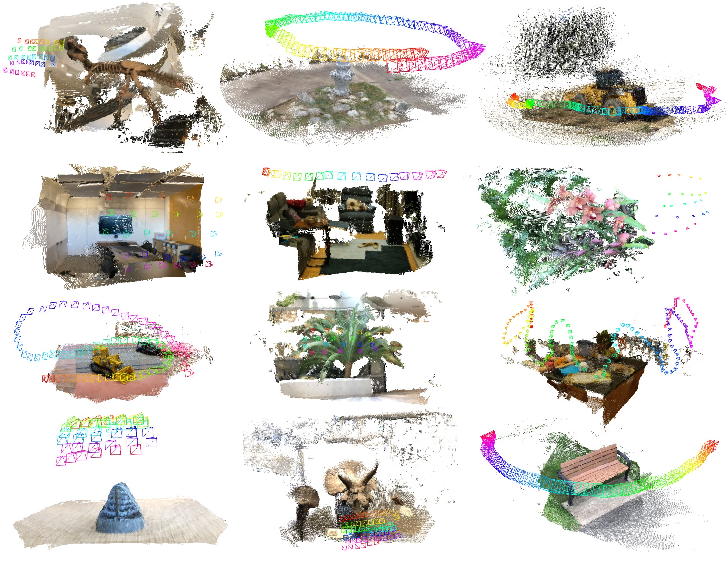
\includegraphics[width=\linewidth,]{figures/pdfs/point_clouds_more_compressed.pdf}
    \caption{\textbf{Additional Point Clouds} Here we plot additional point clouds across the Tanks and Temples, LLFF, Mip-NeRF360, and CO3D datasets.}
    \label{fig:add_clouds}
\end{figure}

